\chapter{Literature Review}
\section{Ascidian tail development}

The notochord is one of the most distinguishing characteristics of chordates. In their adult form ascidians and their vertebrate cousins have no resemblance, however during development they have similar body plans featuring the notochord \cite{jeffery_minireview_2002}. Ascidians are known for the bilateral and invariant cell cleavage. Their development is well described up to the gastrulation stage \cite{nishida_cell_1983,nishida_cell_1985,nishida_cell_1987}. Like vertebrate chordates such as xenopus ascidians depend on maternally localized determinants to regulate cell moments and division, however the location and identity of these determinants are different although the development of the early body plans are similar \cite{lemaire_ascidians_2008}. Solitary ascidians notochords typically come from two cell lineages, the primary notochord derive from the ``A'' blasomere and the secondary notochord comes from the ``B'' blastomere \cite{nishida_cell_1983} which can be identified by the 4-cell embryonic stage. At the 4-cell stage the blastomeres are labeled in Conklin \cite{conklin_organization_1905} convention; ``a'' and ``A'' for the anterior animal and vegetal blastomeres, respectively and ``b'' and ``B'' for the posterior animal and vegetal blastomeres, respectively. Although the notochords cells have been traced back to the 4-cell stage, notochord inductions does not occur until the 32-cell stage. By the 64-cell stage there are 10 notochord cell precursors, the 8 primary precursor notochord cells\textemdash A lineage\textemdash are identifiable and no longer multipotent, while the 2 secondary notochord cells are not restricted until the 110-cell stage \cite{nishida_cell_1985,yasuo_ascidian_1994,yasuo_conservation_1998,lemaire_unfolding_2009}. Two additional stages of cell division occur, one at gastrulation and one at neurulation, ending with 40 notochord cells, which is typical of most solitary ascidian tadpole larvae \cite{conklin_organization_1905}. At the onsite of neurulation the notochord begins to form, this process includes the closing of the neural tube and posterior movement of the notochord and muscle cells, followed by the mediolateral convergence of the notochord cells to the midline then the polarization and intercalate of the cells through a process known as convergence and extension\cite{swalla_mechanisms_1993}. At this point the larval tail is constructed of a notochord flanked by 3 rows of muscles on each side, and both notochord and muscle cell derive from the same blastomeres \cite{nishida_cell_1985}. The arrangement of the notochord cells is a stochastic process, the anterior 32-cells\textemdash primary notochord cells\textemdash are always formed by the A7.3 and A7.7 blastomere and the posterior most 8\textemdash secondary\textemdash notochord cells are always formed by the B8.6 blastomere, but the ordering of the 32 most anterior is not determinate, cells from both the A7.3 and A7.7 intercalate in a random order (Figure~\ref{fig:noto_cells})\cite{nishida_cell_1983,nishida_cell_1985,miyamoto_formation_1985, swalla_mechanisms_1993,kourakis_one-dimensional_2014}. This process, along with muscle cell are the causes the larval tail to form \cite{miyamoto_formation_1985, jeffery_factors_1992,swalla_mechanisms_1993}.

\begin{figure}[tbp]
\centering
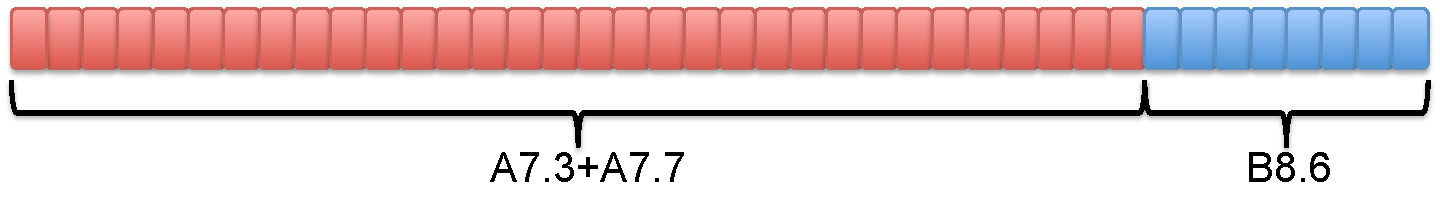
\includegraphics[scale=0.5]{figures/noto_cells.pdf}
\caption{\textbf{Notochord cells.}The primary notochord cell (blue) also known as the A-lineage are specified at the 64-cell stage. There are a total of 32 primary notochord cell that come from the A7.3 and A7.7 blastomere, and the intercalation of the cell happen in a semi-random stochastic manner.The secondary notochord cells (red) comes from the B8.6 blastomere and are specified at the 110-cell stage, one cell division after the primary notochord cells.}
\label{fig:noto_cells}
\end{figure}

Although a tailed larvae is typical of most ascidians, several species with in the Stolidobranchia order have individually undergone tail-loss, many of which fall in the Molgulidae \cite{berrill_studies_1931, jeffery_evolution_1999, huber_evolution_2000, maliska_molgula_2010}. The tail-less\textemdash anural\textemdash species develop in a similar manner and are indistinguishable from their tailed\textemdash urodele\textemdash counterparts up to late gastrulation \cite{berrill_studies_1931, swalla_interspecific_1990, jeffery_factors_1992}. Anural ascidians lack several urodele features including an intercalated and extended notochord, differentiated muscle cells and the otilith sensory organ. The absence of differentiated muscles cells and intercalated notochord are the cause for the lack of tail in these species \cite{miyamoto_formation_1985, swalla_interspecific_1990}. The development of several tail-less species have been studied. \textit{M. tectiformis} notochord cells do not divide again after the 10 precursor cells are formed and \textit{M. occulta} stops dividing after 20 cells \cite{jeffery_evolution_1999}. The same occurs in \textit{M. bleizi}, however after the 20 notochord cells are formed, the embryo attempts to make a tail but never completes the process \cite{swalla_novel_1993}. It has also been shown that chordate embryos without fully developed notochord and/or muscle cells do not fully elongate or fail completely to develop a tail \cite{jeffery_evolution_1999,takada_brachyury_2002,stemple_structure_2005}. 
Seeing that most ascidians have tailed larvae and that the tail can be restored through the use of interspecies hybrids, the lack of tail has been shown to be a loss of function. \textit{M. oculata} and \textit{M. occulta} both of the Roscovita clade have been shown to produce hybrids in lab conditions. Of the known \textit{Molgula} species \textit{M. occulta} and \textit{M. oculata} are the only two that can hybridize. Although \textit{M. occulta} and \textit{M. oculata} have been found to dwell in the same habitat, hybrids have not been found in nature and have only been produced in lab conditions. Fertilizing \textit{M. oculata} eggs with \textit{M. occulta} sperm in most cases produce embryos with fully formed tails. The reciprocal hybrid produces an embryo with 20 notochord cells like \textit{M. occulta}, however the notochord cells converge and extent like \textit{M. oculata} \cite{swalla_interspecific_1990}. The ascidian tail has been shown to form in the presence of notochord and the absence of muscles cells \cite{miyamoto_formation_1985} and the hybrid tail is not flaked by muscles as that of tail species \cite{swalla_novel_1993}. However, also it has been shown that embryos that develop urodele features are batch specific, and only in embryos that express the p58 which is associated with cytoskeleton are urodele features restored \cite{swalla_identification_1991,jeffery_factors_1992}. It has also been shown that in hybrid embryos in which urodele features were restored, the number of cells that express acetylcholinesterase (AChE) in a vestigial muscle cell lineage increased in comparison to hybrids lacking urodele features and \textit{M. occulta} \cite{jeffery_evolutionary_1991}. This along with evidence that with may have been, the ancestral notochord\textemdash the axochord\textemdash is muscle based \cite{lauri_development_2014}, shows strong evidence for the need of both notochord and muscles cells for the formation of the ascidian tail. 

\section{Brachyury has been shown to be the  }

\textit{Brachyury} a T-box transcription factor, has been identified to be essential for notochord development \cite{yasuo_conservation_1998}. The notochord induction is regulated by the \textit{FGF/MAPK/Ets} signaling cascade \cite{minokawa_binary_2001}. Where the A6.2 and A6.4 notochord/nerve cord precursors are induced by \textit{FGF9/16/20} at the 32-cell stage, just after the 7th cell cleavage \cite{satoh_ascidian_2001}. It was observed from isolation experiments that notochord/nerve cord precursors that loss \textit{FGF9/16/20} competence at the 32-cell stage assume the default nerve cord cell fate, the converse is true for presumptive nerve cord blastomeres that are introduce to \textit{FGF}, they forgo their default nerve cord fate and choose the notochord fate \cite{yasuo_conservation_1998,minokawa_binary_2001}. If \textit{FGF9/16/20} is not present at the 32 cell stage competence is lost, \textit{bra} is not induced and the notochord can no longer from \cite{nakatani_basic_1996,nakatani_duration_1999}. This is because \textit{MAPK} is not activated and the induction of \textit{bra} and repression of \textit{FoxB} are not carried out \cite{hashimoto_transcription_2011}. Without the repression of \textit{FoxB TF} the notochord cell fate is repressed through the repression of \textit{bra}. It has been observed in \textit{H. roretzi} that \textit{FoxB} represses the activation of \textit{bra} predominately through the binding of Fox BS1 (GCACTGA\textit{ACAAACA}TACATAG). \textit{FoxB} is activated by \textit{ZicN} and present in both nerve cord and notochords precursors, however is repressed by \textit{MAPK} in the notochord cell lineage at the 64-cell stage \cite{hashimoto_transcription_2011}. \textit{MAPK} is thought to be repressed by \textit{Ephin} which is one of the key differences between notochord and nerve cord determination. At this point \textit{bra} is expressed first weakly in the at the 64-cell stage in the notochord/nerve chord precursors \cite{yasuo_ascidian_1994} and unlike other chordates, in ascidians \textit{bra} is only expressed in the notochord cells \cite{yasuo_function_1993,corbo_characterization_1997,hotta_temporal_1999,takada_brachyury_2002}. Although \textit{bra} is necessary, its presence does not guarantee a tail. \textit{M. occulta} and \textit{M. tectiformis}, two tailless \textit{Molgula}, both express \textit{bra}. In both cases \textit{bra} expression stop earlier than that of \textit{M. oculata}, but produce different results. \textit{Bra} is expressed in the 10 precursor notochord cells in \textit{M. occulta}, another round of cell division occurs which does not in \textit{M. tectiformis}.  In these two species of \textit{Molgula} muscle actin became pseudo genes, however the mutation in the muscle actin genes are not the same \cite{swalla_novel_1993,jeffery_evolution_1999}. \textit{Manx} is another gene identified to be important for tell development in \textit{Molgula}, and is lowly expressed in \textit{M. occulta}, and has been shown to restore the hybrid tail \cite{swalla_requirement_1996, swalla_multigene_1999}. 
  
After cell specification, the notochord cells must converge, intercalate and extend. The Planar Cell Polarity (PCP) pathway is involved in cell movement during this process and mutations in \textit{prickle}\textemdash a known PCP gene\textemdash have shown to cause a shortened ascidian tail affecting both the mediolateral intercalation and the elongation of the ascidan tail \cite{jiang_ascidian_2005}. The \textit{pk} mutant \textit{aimless} produces a truncated tail, however the polarity of the nuclei are present, showing that prickle does not establish polarity with in the cell but polarity between cells, acting in a local manner and perhaps their is a global organizer \cite{jiang_ascidian_2005,kourakis_one-dimensional_2014}. However, even in the absence of the PCP pathway considerable convergence and elongation of the notochord was observed in Ciona, driven by a presumed boundary effects \cite{veeman_chongmague_2008}.

Many of the upstream genes and transcription factors that interact with \textit{bra} has been studied in fair detail, through known-outs, and cell isolation experiments. Not as much detail is known about the downstream genes regulated by \textit{bra}. On larger scale subtractive screening was done to identify genes downstream of \textit{bra}, 39 genes were initially found \cite{hotta_temporal_1999}. An attempt to characterize a number of these genes have been made, identifying functions such as extracellular matrix components (\textit{cadherin 8, entactin, fibronectin, laminin $alpha$1, $alpha$4, and $beta$1, and thrombospondin}, genes involved in cell shape and polarity (\textit{pk, trop, ERM, ACL}), axon guidance (\textit{netrin, semaphorin 3A}), amongst a host of other biological processes \cite{hotta_characterization_2000,hotta_brachyury-downstream_2007,kugler_evolutionary_2008}. 

\textit{Oikopleura} which are in the same subphyla\textemdash tunicates or urochordates\textemdash also develops in a typical chordate manner with a notochord and has a compact genome, however, in Larvacean there are 20 notochord cells \cite{seo_miniature_2001,denoeud_plasticity_2010}. \textit{Oikopleura} retains its tail during its adult life stage and at this point \textit{bra} is not expressed in the adult notochord, however, \textit{bra} is expressed in the same manner in the developing larval notochord as ascidians \cite{bassham_brachyury_2000,nishida_development_2008}. When comparing gene networks, \textit{Oikopleura} did not exhibit the same mechanism for tail development as \textit{Ciona}, of the 50 bra target genes previously identified cite only 26 of them had orthologs, almost 50\% of the genes were not present \cite{kugler_evolutionary_2011}. Of the genes that did show homology, expression ranged from notochord specific to tail including possible notochord, to tissues that were clearly not the notochord.


\section{Assembling and analyzing data}
One of the major advances in science in the past 20 years was the implementation of sequencing technologies. These technologies allowed us to examine problems in ways not previously possible. The first wave was Sanger sequencing in the 1986, but was not broadly used until 10 years later. Another technology, mircoarrays, which became popular starting in the mid '90s, allow us to look at a wide spectrum of genes and understand relative expression within a sample. Kobayashi et al. \cite{kobayashi_differential_2013} isolated and analyzed gene expression in notochord (A7.3+A7.7) and nerve cord (A7.4+A7.8) precursors using microarrays. This study was able to identify 106 genes expressed in the notochord precursor and 68 expressed in the nerve cord precursor at the 64-cell stage. Of these the genes, 36 notochord genes and 25 nerve chord genes were confirmed via Whole Mount In Situ Hybridization in the respective cells. This demonstrates the power of this technique, however, prior knowledge is needed. \textit{C. intestinalis} was sequenced using sanger sequencing, and is well assembled and most well annotated \cite{dehal_draft_2002}. In addition to long reads (Sanger) scaffolding was done using experimental data\cite{satou_improved_2008}. Sanger sequencing able to sequence whole genomes without the need of prior knowledge to identify novel genes but is costly and time consuming\cite{metzker_emerging_2005,liu_comparison_2012}. 

Sanger was the $1$\textsuperscript{st} generation of sequencing technologies, and currently both $2$\textsuperscript{nd} and $3$\textsuperscript{rd} generation are in use, with Roche 454, Ion Torrent, Illumina and PacBio are the most wide spread. These technologies are far easier to produce data and much less costly than sanger sequencing \cite{metzker_emerging_2005}. There are many trade-offs for each of the technologies, cost per MB, sequencing time, prep cost, error rate and sequencing bias; 454 and PacBio have longer reads than Illumina and Ion Torrent, 800 bp and 1+kbp, respectively. However, both Illumina and Ion Torrent's short reads are cheaper to generate, produce more reads and better for counting, in addition to PacBio having a high error rate \cite{glenn_field_2011}. Illumina and Ion Torrent have the best error rates and while Ion Torrent calls more more Single nucleotide polymorphisms, it also calls more false positives.  For this reason, amongst other Illumina is the most used because it is the most versatile and preforms the best in general \cite{quail_tale_2012}. This drop in price and produced many of the assembled genomes within the Tuncata phyla. Outside of this project there are eight tunicate genomes assembled; \textit{C. intestinalis}, \textit{C. savignyi}, \textit{Oikopleura dioica}, \textit{Botryllus schlosseri}, \textit{Halocynthia uranium}, \textit{H. foretzi}, \textit{Phallusia fumigata}, and \textit{P. mammilata}, but no \textit{Molgula} genomes. 
